% -----------------------------------------------------------------------------------------------------------------------------------------------
% -----------------------------------------------------------------------------------------------------------------------------------------------

% =============================================================================
% = PREAMBULE ET PAGE DE GARDE : NE RIEN MODIFIER ICI SANS UNE BONNE RAISON ! =
% =============================================================================

% -----------------------------------------------------------------------------------------------------------------------------------------------
% -----------------------------------------------------------------------------------------------------------------------------------------------

\documentclass[a4paper,11pt]{article}

\usepackage[francais]{babel}
\usepackage[utf8x]{inputenc}
\usepackage[colorlinks,breaklinks,naturalnames,linkcolor=black,citecolor=black,menucolor=black,pagecolor=black,urlcolor=blue,pagebackref]{hyperref}
\usepackage[babel]{microtype}
\usepackage[tt={oldstyle=false,proportional=false,variable=false}]{cfr-lm}
\usepackage[margin=3.5cm]{geometry}
\usepackage{setspace,booktabs,rotating,placeins}
\usepackage[table,xcdraw]{xcolor}

% Création de 2 styles d'en-têtes et pieds de page : 1 pour le corps du texte et un pour lapage de garde et la table des matières
\usepackage{etoolbox,lastpage,fancyhdr}

\fancypagestyle{main}{%
  \fancyhead[L]{\emph{Université de La Rochelle}}
  \fancyhead[C]{}
  \fancyhead[R]{\emph{Master SPE}}
  \fancyfoot[L]{\emph{Règlement des études 2014--2018}}
  \fancyfoot[C]{}
  \fancyfoot[R]{\thepage\ / \pageref{LastPage}}
  \renewcommand{\headrulewidth}{0.4pt}
  \renewcommand{\footrulewidth}{0.4pt}
}
\fancypagestyle{plain}{%
  \fancyhf{}%
  \fancyfoot{}%
  \renewcommand{\headrulewidth}{0pt}%
  \renewcommand{\footrulewidth}{0pt}%
}

\appto\frontmatter{\pagestyle{plain}}
\appto\mainmatter{\pagestyle{main}}



\title{Règlement des études\\ Master Sciences Pour l'Environnement}
\author{Sciences, Technologie et Santé\\Sciences Humaines et Sociales\\Droit Économie Gestion}
\date{2014--2018}



\begin{document}

\frontmatter

\maketitle

\onehalfspace

\begin{center}
\fbox{\parbox{\textwidth}{Le master délivré par l'université de La Rochelle est un diplôme national.
Le présent règlement des études s'inscrit dans le cadre règlementaire national défini par les textes suivants :
\begin{itemize}
	\item Code de l'éducation
	\item Arrêté du 9 avril 1997 relatif au diplôme d'études universitaires générales, à la licence et à la maîtrise
	\item Arrêté du 25 avril 2002 relatif au master
	\item Arrêté du 11 avril 2012 habilitant l'université de La Rochelle à délivrer ses diplômes de master
	\item Arrêté du 22 janvier 2014 fixant le cadre national des formations conduisant à la délivrance des diplômes nationaux de licence, de licence professionnelle et de master.
\end{itemize}
Ce cadre réglementaire est complété par la charte des examens de l'université de La Rochelle.
Afin de préserver sa mission d'enseignement, l'ULR prévoit à tout moment de l'année la possibilité de déroger à tout ou partie des articles du présent règlement en cas de pandémie constatée par l'autorité administrative compétente.}}
\end{center}

\noindent Avis des conseils d’UFR le 5 juin 2014 (FLASH), le 26 juin 2015 (PST) et le 9 juillet 2015 (DROIT/GESTION).\\

\noindent Adopté en Commission de la Formation et la Vie Universitaire le \ldots{}

\clearpage
\tableofcontents
\clearpage

\mainmatter

% -----------------------------------------------------------------------------------------------------------------------------------------------
% -----------------------------------------------------------------------------------------------------------------------------------------------

% ==========================================================================================
% = LE CORPS DU DOCUMENT COMMENCE ICI : NE RIEN MODIFIER AU-DESSUS SANS UNE BONNE RAISON ! =
% ==========================================================================================

% -----------------------------------------------------------------------------------------------------------------------------------------------
% -----------------------------------------------------------------------------------------------------------------------------------------------

\section{Inscriptions}\label{Inscriptions}
\subsection{Accès}\label{Acces}
\setcounter{page}{1}

L'accès à la 1\iere{} année de master est ouvert aux étudiants ayant obtenu :
\begin{itemize} 
\item soit un diplôme national conférant le grade de licence dans un domaine compatible avec celui du diplôme national de master ; l'accès de l'étudiant titulaire de la licence, dans le même domaine, est de droit pour les 60 premiers crédits européens
\item soit une validation prévue aux articles L. 613-3, L. 613-4 et L. 613-5 du code de l'éducation.
\end{itemize}

L'accès à la 2\ieme{} année de master est ouvert aux étudiants ayant obtenu les 60 crédits ECTS de la 1ère année d'un master compatible. L'admission est prononcée par le directeur de la composante par délégation du président de l'université, sur proposition du responsable de la formation.


\subsection{Niveau de langue requis pour les étudiants étrangers}\label{langue}
Sauf dérogation, le niveau de langue requis pour l'inscription des étudiants étrangers est B2 pour une inscriptions dans les parcours Géosciences et Géophysique du Littoral (GGL) et Géographie Appliquée à la Gestion des Littoraux (GAGL), et C1 pour les parcours Management Environnemental (ME) et Gestion de l'Environnement et Écologie Littorale (GEEL).

\subsection{Inscription administrative}\label{InsciprtionAdministrative}

L'inscription administrative est annuelle et a lieu auprès du service des études et de la vie étudiante (SEVE). Les conditions d'inscription administrative dans chaque année d'études sont définies dans la section~\ref{Progression}.

La date limite d'inscription à l'université de La Rochelle est fixée par décision du président de l'université.
Les deux types d'inscription possibles sont :
\begin{itemize}
\item l'inscription principale
\item l'inscription complémentaire : inscription prise en plus de l'inscription principale pour obtenir un diplôme différent.
\end{itemize}


\subsection{Inscription pédagogique}\label{InscriptionPeda}

\subsubsection{Généralités}

L'inscription pédagogique consiste notamment à formuler les choix de parcours et d'enseignements : langue vivante 2, matières optionnelles, mise en place d'un régime particulier\ldots{} 
L'inscription pédagogique est faite au début de chaque semestre, avec possibilité de modifications au plus tard dans les 15 jours qui suivent le début de la première inscription pédagogique de l'enseignement concerné, sauf dérogation accordée par le responsable des études.
Dans le cas où une inscription administrative tardive ne permet pas le respect de la condition ci-dessus, l'inscription pédagogique doit être faite dans la semaine suivant l'inscription administrative, sans possibilité de modification ultérieure.

Les demandes de modification d'inscriptions pédagogiques doivent être formulées auprès :
\begin{itemize}
\item du secrétariat du département de Biologie du bâtiment Orbigny (2ème étage, bureau B22) pour les parcours GGL et GEEL
\item du secrétariat du Master SPE du bâtiment Flash 2 (2ème étage, bureau D211) pour le parcours GAGL
\item du secrétariat du Master SPE à l'IAE (Institut d'Administration des Entreprises) pour le parcours ME
\end{itemize}

\subsubsection{Cas particuliers : auditeurs libres}
Les auditeurs libres n'ont pas d'inscription pédagogique. Ils ne sont autorisés qu'à assister aux cours magistraux de leur choix. Ils ne peuvent pas assister aux TP ni aux TD et ne sont pas autorisés à se présenter aux examens.

\section{Organisation des études}\label{Organisation}

\subsection{Organisation temporelle de la formation}\label{Temporel}

Aucun enseignement ni aucune modalité d'évaluation n'a lieu pendant les dates de congés universitaires fixées chaque année par le conseil d'administration. Les activités physiques, sportives et d'expression sont organisées le jeudi après-midi, ainsi que les éventuelles épreuves les concernant, à l'exclusion de tout autre type d'enseignement et épreuve. Les emplois du temps ménagent une pause méridienne d'au moins une heure, dans le créneau de 11h45 à 14h. Ces règles ne s'appliquent pas aux stagiaires de la formation continue ni, le cas échéant, aux étudiants suivant la formation à distance.

Les calendriers de la formation sont détaillés à la section~\ref{Calendrier}.

\subsection{Parcours, UE, EC et ECTS}

Le master est organisé en quatre semestres notés S1 à S4. Chaque semestre est composé d'Unités d'Enseignement (UE). Chaque UE contient un ou plusieurs Éléments Constitutifs (EC). Les parcours sont organisés en UE pouvant contenir des EC obligatoires et des EC optionnels disciplinaires.

Des crédits ECTS (European Credits Transfer System ou système européen de transfert de crédits) sont affectés aux UE et aux EC et sont répartis par points entiers. Le master sanctionne un niveau validé par l'obtention de 120 crédits ECTS à raison de 30 ECTS par semestre, au-delà du grade de licence.

Le master mention \textbf{Sciences Pour l'Environnement} (SPE) comporte 4 parcours.
\begin{itemize}
\item Gestion de l'Environnement et Écologie Littorale : \textbf{GEEL} (UFR Sciences Fondamentales et Sciences Pour l'Ingénieur)
\item Géosciences et Géophysique du Littoral : \textbf{GGL} (UFR Sciences Fondamentales et Sciences Pour l'Ingénieur)
\item Géographie Appliquée à la Gestion des Littoraux : \textbf{GAGL} (UFR des Lettres, Langues, Arts et Sciences Humaines)
\item Management Environnemental : \textbf{ME} (UFR Droit, Science Politique et Gestion)
\end{itemize}

\subsection{Types d'enseignement}\label{TypesEnseignements}

Quatre types d'enseignements sont assurés :
\begin{itemize}
\item Les cours magistraux (CM) : ils sont à la base de l'enseignement et réunissent l'ensemble des étudiants.
\item Les travaux dirigés (TD) : ils illustrent et complètent le cours par des exercices d'application. La participation active des étudiants, réunis en groupe, y est essentielle, en particulier sous la forme de présentations orales ou de commentaires de documents.
\item Les travaux pratiques (TP) : ils permettent d'offrir dans certains enseignements le lien entre théorie et application.
\item Les stages et projets : ils offrent l'occasion à l'étudiant de se livrer à un travail personnel dans un environnement professionnel ou de recherche. Ils offrent à l'étudiant un contact privilégié avec le milieu professionnel auquel il se destine et lui permettent d'en apprécier les spécificités.
\end{itemize}


\subsection{Régime de présence, assiduité}
La présence aux enseignements et aux examens, quelle qu'en soit la forme, est obligatoire.
Des dérogations peuvent être prévues dans le cadre de modalités pédagogiques et d'évaluation adaptées aux étudiants à statut spécifique (voir section~\ref{StatutSpe}). Aucune dispense d'assiduité ne peut être accordée à un étudiant boursier, hormis dans le cas d'une situation de handicap (voir section~\ref{Handicap}).
En dehors de ces dérogations, toute absence doit être justifiée auprès du service suivant :
\begin{itemize}
\item du secrétariat du département de Biologie du bâtiment Orbigny (2ème étage, bureau B22) pour les parcours GGL et GEEL
\item du secrétariat du Master SPE du bâtiment Flash 2 (2ème étage, bureau D211) pour le parcours GAGL
\item du secrétariat du Master SPE à l'IAE (Institut d'Administration des Entreprises) pour le parcours ME
\end{itemize}

L'étudiant arrivant en retard ou qui perturbe le déroulement d'un enseignement ou d'un examen peut être exclu ; il est alors considéré comme absent.
Les justificatifs d'absence doivent être transmis dans la semaine à compter du premier jour de l'absence. Aucun justificatif ne sera admis en dehors de ce délai et l'absence sera alors considérée comme injustifiée.
Il appartient au responsable de la formation d'apprécier la validité des justificatifs fournis pour les absences aux enseignements, et au président du jury en ce qui concerne les absences aux épreuves, sauf s'il s'agit d'un certificat médical du service de santé universitaire, qui vaut justification de l'absence.

\subsection{Stages}
\subsubsection{Organisation, durée}
Le master comprend des périodes de stage en milieu professionnel, d'une durée indiquée ci-dessous, donnant droit à l'obtention d'ECTS et ayant un lien avec l'un au moins des enseignements dispensés. Tout stage fait l'objet d'un encadrement, d'un suivi particulier et d'une évaluation.

La durée du stage pour les parcours GEEL, GGL et GAGL est de 6 semaines minimum, et de 8 à 10 semaines pour le parcours ME. Pour les parcours GAGL et ME, les étudiants du M1 ont le choix entre le stage ou la rédaction d'un mémoire de recherche. Pour les parcours GGL et GEEL, le stage est obligatoire. 

\subsubsection{Évaluation}
Seuls les stages comptant pour l'obtention du diplôme font l'objet d'une validation dans le cursus de formation de l'étudiant. En cas de réussite à l'évaluation du stage, cette validation se traduit par la délivrance de 9 crédits ECTS pour le parcours ME et de 3 crédits ECTS pour les autres parcours du master. L'étudiant doit produire :
\begin{itemize}
	\item un rapport écrit (50\% de la note). Le rapport devra être restitué en deux exemplaires à l'issue du stage, impérativement à la date indiquée par le responsable des stages. Le rapport est noté sur vingt.
	\item une soutenance orale (50\% de la note). Les étudiants devront faire une présentation orale devant un jury comprenant au moins deux enseignants de l'université. Le maître de stage pourra y participer s'il le souhaite, mais seulement à titre consultatif. La soutenance est notée sur vingt. La présentation orale durera 10 minutes (pour les parcours GAGL, GGL et GEEL) et sera suivie d'une période de 10 minutes pendant laquelle le candidat devra répondre à une série de questions posées par les membres du jury.
\end{itemize}

Concernant les étudiants du parcours ME, les consignes relatives à la rédaction du rapport de stage et à sa soutenance sont fournies dans le guide de stage de la formation.

\textsc{Cas exceptionnel} : les étudiants effectuant leur stage hors France Métropolitaine et ne pouvant raisonnablement être présents pour la soutenance, pourront réaliser celle-ci en visio-conférence. En cas d'impossibilité, ils seront évalués uniquement sur le rapport écrit et l'évaluation du maître de stage.

\subsubsection{Structure d'accueil et convention}

L'étudiant a la charge de trouver sa structure d'accueil. La Maison de la Réussite et de l'Insertion Professionnelle (MRIP) de l'université peut l'aider dans ses démarches de recherche de stage (s'adresser au bureau d'aide à l'insertion professionnelle des étudiants - BAIPE).

Les étudiants doivent obligatoirement effectuer une demande de convention de stage via l'application informatique prévue à cet effet qui leur est accessible sur l'Environnement Numérique de Travail (ENT) de l'Université de La Rochelle.
Une convention de stage est délivrée à l'étudiant une fois l'accord du responsable des stages et du tuteur pédagogique, et après avoir été dûment signée par le directeur de l'UFR.
Le stage ne peut pas commencer avant la signature de la convention par l'étudiant, le représentant de l'organisme d'accueil du stage et le directeur de l'UFR.
Toute convention signée par l'étudiant l'engage définitivement. Un manquement à cette règle entraînera la non validation du stage.

\section{Organisation des contrôles des connaissances}\label{cc}

Deux sessions de contrôle des connaissances et aptitudes sont organisées : une session initiale et une session de rattrapage après une première publication des résultats. Seuls les étudiants inscrits administrativement et pédagogiquement à l'Université de La Rochelle sont admis à se présenter aux examens et peuvent les valider.

\subsection{Convocation aux examens terminaux}\label{exam}
La convocation aux épreuves écrites et orales des examens est réalisée par voie d'affichage, avec indication de la date, de l'heure et du lieu d'examen. Le délai entre l'affichage tenant lieu de convocation et la date des épreuves écrites de l'examen est de quinze jours.
Dans le cas particulier des étudiants ne pouvant pas avoir régulièrement accès à l'affichage (dispensés d'assiduité, handicapés, voir section~\ref{Handicap} sur les étudiants à statut spécifique), une convocation individuelle est adressée par courrier électronique à l'adresse électronique fournie par l'ULR lors de l'inscription.

\subsection{Accès des candidats aux salles d'examen}
Pour être autorisé à composer, un étudiant doit :
\begin{itemize}
	\item Présenter sa carte d'étudiant ou, à défaut, son certificat de scolarité et une pièce d'identité.
	\item Se présenter à l'épreuve avant l'ouverture des enveloppes contenant le sujet. L'accès de la salle d'examen est interdit à tout candidat qui se présente après l'ouverture de l'enveloppe contenant les sujets. Exceptionnellement, lorsque le retard est dû à un cas de force majeure et si ce retard est inférieur au quart de la durée de l'épreuve, le surveillant peut autoriser l'accès du candidat retardataire. Aucun temps supplémentaire ne sera accordé au candidat concerné. Mention du retard et des circonstances seront portées sur le procès-verbal d'épreuve.
\end{itemize}

Les étudiants ne conservent avec eux que le matériel éventuellement autorisé et notifié sur le sujet de l'épreuve ou prévu dans l'arrêté d'aménagement d'épreuve pour les étudiants qui en bénéficient. Notamment, les téléphones portables ne sont pas autorisés même en qualité d'horloge. Les sacs, porte-documents, cartables, téléphones, écouteurs, etc sont placés à l'endroit indiqué par les surveillants de salle.

En cas de retards prévisibles d'étudiants pour accéder aux salles d'examen (grève des transports par exemple), à moins que la réglementation de l'examen ne s'y oppose, le président du jury du semestre concerné ou son représentant peut décider de retarder le commencement de l'épreuve ou de la reporter à une date ultérieure.
Sauf cas de force majeure --- c'est-à-dire événement non seulement irrésistible mais aussi imprévisible --- dès que les sujets sont distribués, aucun candidat n'est autorisé à se déplacer et à quitter la salle avant la fin du premier tiers de la durée de l'épreuve, même s'il rend une copie blanche.
Si les candidats qui demandent à quitter provisoirement la salle y sont autorisés, ils ne sortent qu'un par un et accompagnés d'un surveillant.
L'étudiant ne peut user d'aucun moyen de communication (téléphone portable, etc.), ni au cours de l'épreuve, ni à l'occasion d'une sortie momentanée.
En cas d'annulation d'une épreuve après que celle-ci s'est tenue en tout ou partie, seuls les étudiants ayant été présents à l'épreuve annulée peuvent participer à l'épreuve de remplacement. Le même dispositif pourra s'appliquer aux épreuves de contrôle continu à l'initiative de l'enseignant.

\section{Modalités de contrôle des connaissances}
Les modalités de contrôle des connaissances définies conformément à l'article L.~613-1 du code de l'éducation réglementent les conditions d'obtention de chacun des diplômes délivrés par l'Université de La Rochelle. Les modalités de ce contrôle tiennent compte des contraintes spécifiques des étudiants accueillis au titre de la formation continue. Elles comportent l'indication du nombre d'épreuves, de leur nature, de leur durée, de leur coefficient ainsi que la répartition éventuelle entre le contrôle continu et le contrôle terminal et la place respective des épreuves écrites et orales.

\subsection{Types d'épreuves}
Chaque semestre de master est validé sur la base de la moyenne générale des notes obtenues aux UE auxquelles les étudiants sont inscrits administrativement et pédagogiquement.
Les aptitudes et l'acquisition des connaissances sont appréciées par un contrôle continu et/ou par un examen terminal.
Selon les modalités prévues pour chaque EC, le contrôle des connaissances repose sur une ou plusieurs épreuves dont les résultats participent au calcul de la moyenne de l'EC. Ces épreuves sont les suivantes :
\begin{description}
	\item[le contrôle continu] il repose sur des travaux et exercices présentés par écrit et/ou oralement, mais aussi sur l'assiduité et la participation, selon l'organisation propre à chacun des EC . L'organisation du contrôle continu est expliquée par chacun des enseignants dès leur première séance d'enseignement.
	\item[l'examen terminal] il comprend une épreuve écrite ou orale organisée en fin d'enseignement. Pour les épreuves écrites, l'anonymat des copies est strictement respecté. Quand il est prévu, l'examen terminal est obligatoire.
	\item[l'évaluation sur dossier, projet, rapport, mémoire] lorsqu'elle est prévue dans l'organisation d'un EC, elle est obligatoire.
	\item[le stage] le stage ou mémoire doit faire l'objet d'une soutenance et/ou d'un rapport. Les modalités et conditions d'évaluation du stage doivent être explicitement transmises aux étudiants.
\end{description}

\subsection{Validation des EC, UE et semestres}\label{Validation}
\subsubsection{Validation d'un EC}
Un EC ne peut être validé que si les éventuelles absences injustifiées aux enseignements de cet EC (CM, TD, TP) ne sont pas supérieures à 20 \%.
Si la condition d'assiduité définie ci-dessus est respectée, un EC est acquis :
\begin{itemize}
	\item dès lors que la moyenne des notes obtenues dans cet EC est égale ou supérieure à $10/20$.
	\item par compensation au sein d'une UE acquise, quel que soit le mode d'acquisition de l'UE, à condition que la note moyenne de l'EC soit supérieure ou égale à $7/20$.
	\item Contrairement aux autres EC, les EC stage et mémoire ne sont pas pris en compte dans la compensation.
\end{itemize}

La validation de l'EC emporte l'acquisition des crédits correspondants. Il est définitivement acquis et capitalisé, sans possibilité de s'y réinscrire.

\subsubsection{Validation d'une UE}
Une UE est acquise :
\begin{itemize}
	\item dès lors que la moyenne pondérée des EC qui la composent, affectés de leurs coefficients, est égale ou supérieure à $10/20$, et à la condition que la note moyenne de chaque EC soit supérieure ou égale à $7/20$.
	\item par compensation au sein d'un semestre de parcours type.
\end{itemize}

La validation de l'UE emporte l'acquisition des crédits correspondants. Elle est définitivement acquise et capitalisée, sans possibilité de s'y réinscrire


\subsubsection{Validation d'un semestre}

Un semestre est acquis :
\begin{itemize}
	\item dès lors que l'étudiant valide chacune des UE qui le composent (moyenne de chaque UE égale ou supérieure à $10/20$)
	\item ou par compensation entre les différentes UE qui le composent (moyenne des moyennes d'UE affectées de leurs coefficients, égale ou supérieure à $10/20$), hormis pour les UE stage et mémoire qui n'entrent pas dans la compensation.
\end{itemize}

Pour les étudiants ayant fait un semestre à l'étranger, la compensation n'est pas appliquée. Au vu des résultats communiqués par les universités partenaires, les crédits ECTS sont attribués par le jury et sont pris en compte dans la validation du semestre correspondant au séjour à l'étranger.



\subsection{Règles de compensation}
Il est procédé à une compensation semestrielle sur la base de la moyenne générale des notes obtenues pour les diverses UE.
Il n'est procédé à aucune compensation annuelle. L'année est validée si chacun des semestres est acquis selon les règles décrites dans la section~\ref{Validation}.



\subsection{Règles concernant les sessions}
\subsubsection{Première session}
En première session, pour les EC évalués totalement ou en partie en contrôle continu, en l'absence d'une ou plusieurs notes de contrôle continu due à une ou plusieurs absences justifiées, l'enseignant responsable de l'enseignement, avec l'accord du responsable de la formation, détermine, à titre dérogatoire, soit un nouveau mode de calcul de l'EC, soit une nouvelle épreuve pour l'étudiant concerné en remplacement d'un ou des contrôles continus.

\subsubsection{Session de rattrapage}
Si le semestre n'est pas validé à l'issue de la première session, l'étudiant doit se présenter à la session de rattrapage des EC dont la moyenne des notes est inférieure à $10/20$, au sein des UE non acquises. L'étudiant qui ne se présente pas à l'une des épreuves de la session de rattrapage est noté ``absent'' et ne peut valider son semestre.

Il n'est pas possible de participer à la session de rattrapage pour améliorer les résultats des EC déjà validés.

Seuls sont autorisés à se présenter à la session de rattrapage les étudiants présents à la session initiale ou dont l'absence à la session initiale est liée à un événement indépendant de leur volonté. Si cet événement concerne la santé de l'étudiant, il devra être justifié par un certificat médical. Quel que soit le motif invoqué, il appartient au jury d'apprécier la validité des justificatifs fournis, sauf s'il s'agit d'un certificat médical du SDSU, qui vaut justification de l'absence et autorisation à se présenter en session de rattrapage.
Cette restriction ne concerne pas les étudiants relevant d'un régime spécifique (voir section~\ref{StatutSpe} sur les étudiants à statut spécifique).
En principe, aucun étudiant n'est admis à partir en séjour d'études à l'étranger s'il n'a pas validé le semestre précédant la mobilité. Si toutefois, par exception, un étudiant est autorisé à partir avant que les résultats de première session ne soient connus, et s'il ne valide pas son semestre à l'issue de la première session, il devra revenir pour se présenter à la session de rattrapage organisée à l'ULR. Dans le cadre des séjours d'études, l'ULR n'organise aucune session d'examen à l'étranger.

On ne prend pas en compte les notes de contrôle continu dans le calcul du résultat de la session de rattrapage. Le résultat obtenu à la session de rattrapage annule et remplace celui obtenu à la première session. Seules les notes obtenues aux épreuves de session de rattrapage sont prises en compte dans le calcul de la moyenne des EC repassés.

\subsubsection{Régime des absences non justifiées}
En cas d'absence non justifiée à un examen terminal ou une épreuve de contrôle continu, l'étudiant est noté ``absent''. Aucun calcul de moyenne ne peut donc être réalisé ni, par conséquent, aucune compensation. L'année ne peut donc pas être validée.

\subsection{Bonification sport et activités d'expression}

Les étudiants de master pratiquant une activité sportive, culturelle ou d'expression encadrée et notée par le Suapse bénéficient d'une bonification qui s'applique sur leur moyenne annuelle si celle-ci est supérieure à $10/20$. Le nombre de points de bonification est fonction de la note obtenue :

\begin{table}[htpb] 
\begin{center}
    \begin{tabular}{c c}
        \toprule
        Note sur 20 & Bonification\\ 
        \midrule
        10 à 11,99 & 0,10 \\ 
        12 à 13,99 & 0,15 \\ 
        14 à 15,99 & 0,20 \\ 
        16 à 17,99 & 0,25 \\ 
        18 à 20,00 & 0,30 \\ 
        \bottomrule
    \end{tabular} 
\end{center}
\end{table}


\subsection{Délibérations du jury}
Le jury délibère souverainement dans le respect de la réglementation en vigueur.
Le jury de semestre délibère et arrête les notes des étudiants à l'issue de chaque session de chaque semestre. Il se prononce sur l'acquisition des UE, des EC et la validation des semestres de parcours type.
Lors de ses délibérations le jury peut attribuer des points de jury.

À l'issue du semestre 2, le jury de diplôme décide l'attribution du diplôme de maîtrise en appliquant le cas échéant les règles de compensation.
Les résultats peuvent être contestés dans les deux mois à compter de la date de leur publication.


\subsection{Délivrance du diplôme}
Le diplôme de maîtrise est délivré après l'obtention de 2 semestres d'enseignement représentant 60 crédits ECTS. Une attestation de réussite est fournie trois semaines au plus tard après la proclamation des résultats.

Le diplôme de maîtrise est attribué à l'étudiant, à sa demande, lorsque la première année du master est obtenue. Une attestation de réussite est délivrée à la demande de l'étudiant.

La délivrance du diplôme définitif et de l'annexe descriptive au diplôme, réalisée par le Service des Études et de la Vie Étudiante (SEVE) de l'université intervient dans un délai inférieur à six mois après la proclamation des résultats.

Un relevé de notes semestriel est délivré à l'issue des sessions.



\subsection{Retrait des relevés de notes et de l'attestation de réussite}
Sur présentation de leur carte d'étudiant ou d'une pièce d'identité, les étudiants pourront retirer leurs relevés de notes ou leurs attestations de réussites auprès du secrétariat scolarité dont dépend l'étudiant : 
\begin{itemize}
\item secrétariat du département de Biologie du bâtiment Orbigny (2ème étage, bureau B22) pour les parcours GGL et GEEL
\item secrétariat du Master SPE du bâtiment Flash 2 (2ème étage, bureau D211) pour le parcours GAGL
\item secrétariat du Master SPE à l'IAE (Institut d'Administration des Entreprises) pour le parcours ME
\end{itemize}



\subsection{Mention}
Aucune mention n'est attribuée aux semestres, aux UE comme aux EC mais des mentions sont attribuées au niveau des diplômes :
\begin{description}
	\item[Mention ``Très bien'']	 pour une moyenne générale supérieure ou égale à $16/20$
\item[Mention ``Bien''] pour une moyenne générale supérieure ou égale à $14/20$
\item[Mention ``Assez bien''] pour une moyenne générale supérieure ou égale à $12/20$
\item[Mention ``Passable''] pour une moyenne générale supérieure ou égale à $10/20$
\end{description}




\section{Progression}\label{Progression}
\subsection{Inscription en 2\ieme{} année de master}
L'admission en M2 est prononcée par le directeur de la composante par délégation du président de l'université, sur proposition du responsable de la formation.

\subsection{Inscription complémentaire}
Un étudiant inscrit en complémentaire peut suivre les enseignements et se présenter aux examens des EC auxquels il est inscrit administrativement selon les possibilités de l'emploi du temps.


\section{Sanctions disciplinaires}

\subsection{Fraude}
Toute fraude, y compris notamment le plagiat ou la falsification de documents officiels tels que les certificats médicaux, est passible de poursuites disciplinaires et de poursuites pénales. Cette disposition concerne toutes les épreuves que les étudiants sont amenés à passer, quelles qu'en soient la nature et les modalités d'organisation, notamment :
\begin{itemize}
	\item travaux dirigés, travaux pratiques ou examens tant oraux qu'écrits
	\item différentes tâches données aux étudiants dans le cadre du contrôle continu
	\item mémoires
	\item rapports de stage
\end{itemize}

Dans l'attente de la décision de la section disciplinaire, l'épreuve est évaluée dans les mêmes conditions que pour les autres candidats. Le jury ne peut pas attribuer la note zéro en raison d'un soupçon de fraude. Il délibère sur les résultats de l'étudiant suspecté de fraude dans les mêmes conditions que pour tout autre candidat. Cependant, la note obtenue n'est pas communiquée à l'étudiant. Aucune attestation de réussite ni relevé de notes ne peut lui être délivré, aucune inscription dans un établissement d'enseignement supérieur public n'est possible, avant que la section disciplinaire n'ait statué sur son cas.
La sanction encourue en cas de fraude aux examens peut aller jusqu'à l'exclusion définitive de tout établissement d'enseignement supérieur.


\subsection{Atteinte au bon fonctionnement de l'établissement}
Tout usager auteur ou complice d'un fait de nature à porter atteinte à l'ordre ou au bon fonctionnement de l'établissement est passible de poursuites disciplinaires.

\section{Modalités d'enseignement et d'évaluation adaptées aux étudiants à statut spécifique}\label{StatutSpe}
\subsection{Dispositions communes}\label{Communes}
L'Université de La Rochelle offre des modalités pédagogiques prenant en compte les besoins de publics étudiants ayant des contraintes particulières.
Ce régime spécifique inclut des modalités pédagogiques appropriées (aménagements des emplois du temps et des rythmes d'études, choix du mode de contrôle des connaissances, \ldots{}). L'étudiant concerné peut éventuellement bénéficier d'une dispense d'assiduité aux enseignements magistraux, aux travaux dirigés ainsi qu'aux travaux pratiques. L'étudiant peut également demander à bénéficier de l'étalement de la durée de sa formation.

\subsubsection{Sessions d'examen}\label{DispoExam}
Les étudiants concernés bénéficient au besoin des deux sessions d'évaluation. Notamment, si l'étudiant à statut spécifique est empêché de se présenter à la session initiale, il participe avec les autres étudiants à la session de rattrapage qui tient lieu pour lui de session initiale. Dans ce cas, une session de rattrapage spéciale est organisée en juin pour le semestre impair et en septembre pour le semestre pair.
Cette session de rattrapage spéciale de juin ou septembre tient également lieu de session de rattrapage pour les étudiants à statut spécifique qui, s'étant normalement présentés à la session initiale, ont été ensuite empêchés de se présenter à la session de rattrapage normale.
L'étudiant ne peut bénéficier de ce dispositif que si son absence à la session initiale normale ou à la session de rattrapage normale est prévue dans le contrat pédagogique ou justifiée par un certificat médical du Service De Santé Universitaire (SDSU).


\subsubsection{Procédure}
Hormis pour les étudiants présentant un handicap, qui font l'objet d'une procédure spécifique décrite à la section~\ref{Handicap}, il appartient à l'étudiant concerné de solliciter par écrit un rendez-vous avec le responsable de sa formation pour faire état de ses contraintes et rechercher les adaptations que l'université peut rendre possibles en vue de favoriser sa réussite. Un contrat pédagogique est établi à cette fin entre l'étudiant et l'équipe pédagogique. Il vise à favoriser la réussite de l'étudiant. Il récapitule d'une part les aménagements d'études mis en place par les enseignants et d'autre part les engagements pris par l'étudiant. Ce document est systématiquement transmis au service de scolarité de l'UFR concernée.
Pour pouvoir bénéficier d'un aménagement lié à son statut spécifique, l'étudiant doit solliciter par écrit le responsable de sa formation avant le 15 octobre de l'année universitaire au titre de laquelle il demande l'aménagement. Au-delà de cette date, l'université ne peut pas garantir la mise en \oe uvre d'aménagements. Notamment, une demande d'aménagement d'examen ne pourra pas toujours être satisfaite si elle est présentée à une date trop proche de l'examen concerné.
L'étudiant se doit d'avertir le service de scolarité de tout changement de situation dans un délai d'une semaine pour un nouvel examen de cette situation.
Sont notamment mis en place des dispositifs particuliers pour les publics à statut spécifique décrits dans les sections~\ref{Handicap}, \ref{Salarie}, \ref{Sportif}, \ref{Reserviste} et \ref{Elu} (liste non exhaustive).

\subsection{Étudiants présentant un handicap}\label{Handicap}
Les étudiants qui présentent un handicap tel que défini à l'article L. 114 du code de l'action sociale et des familles peuvent bénéficier d'aménagements portant sur :
\begin{itemize}
	\item Les conditions de déroulement des épreuves, de nature à leur permettre de bénéficier des conditions matérielles (accès aux locaux, installation matérielle, adaptation de la présentation des sujets), des aides techniques, des aides humaines (secrétariat, assistance), appropriées à leur situation.
	\item Une majoration du temps imparti pour une ou plusieurs épreuves, qui ne peut excéder le tiers du temps normalement prévu pour chacune d'elles. Toutefois, cette majoration peut être allongée, eu égard à la situation exceptionnelle du candidat, sur demande motivée du médecin du service de santé universitaire .
	\item La conservation, durant cinq ans, des notes à des épreuves ou des unités obtenues à l'un des examens, ainsi que le bénéfice d'acquis obtenus dans le cadre de la procédure de validation des acquis de l'expérience, le cas échéant.
	\item L'étalement sur plusieurs sessions du passage des épreuves.
	\item Des adaptations d'épreuves ou des dispenses d'épreuves.
	\item L'étalement des études.
	\item L'adaptation de l'emploi du temps avec ou pas possibilité d'absences éventuelles excusées.
\end{itemize}

Il appartient à l'étudiant présentant un handicap d'adresser sa demande d'aménagement au Service De Santé Universitaire (SDSU) ou au relais handicap de l'université pour faire état de ses contraintes et rechercher les adaptations que l'université peut rendre possibles en vue de favoriser sa réussite. Le médecin du SDSU et le relais handicap assistent l'étudiant dans ses démarches. Le médecin du SDSU, au vu de la situation de l'étudiant et des informations médicales actualisées transmises à l'appui de sa demande, propose au président de l'université les aménagements nécessaires. Seul le président de l'université est compétent pour décider de ces aménagements. Sa décision est notifiée à l'étudiant par le relais handicap qui en informe la direction de la composante et le service de scolarité concerné pour mise en \oe uvre et notamment l'information du président du jury.
Pour pouvoir bénéficier d'un aménagement lié à sa situation de handicap, l'étudiant doit présenter sa demande avant le 15 octobre de l'année universitaire au titre de laquelle il la présente (sauf situation particulière : handicap temporaire, évolution de l'état de santé en cours d'année). Au-delà de cette date, l'université ne peut pas garantir la mise en \oe uvre d'aménagements. Notamment, une demande d'aménagement d'examen ne pourra pas toujours être satisfaite si elle est présentée à une date trop proche de l'examen concerné.

\subsection{Étudiants exercant une activité salariée ou professionnelle}\label{Salarie}
Un étudiant salarié est une personne qui suit une formation et en même temps, exerce un travail pour lequel il est rémunéré. L'étudiant est lié à son (ou ses) employeur(s) par un engagement au terme duquel il perçoit en contrepartie un salaire. Cet engagement peut être un contrat à temps plein ou à temps partiel pour une période limitée ou indéterminée, ou tout autre document officialisant son engagement.
L'étudiant salarié doit dans un délai d'une semaine suivant le démarrage de son activité (ou reprise des cours si l'activité débute en période de congés), communiquer à la scolarité de son UFR une copie de cet engagement. S'il considère que cette activité soit par son volume, soit par son organisation, influe sur sa capacité à suivre les enseignements ou à assurer le travail personnel nécessaire à la réussite de ses études, il sollicite un rendez-vous avec le responsable de sa formation.
Un éventuel aménagement de l'emploi du temps doit être prévu avant l'absence. Si l'aménagement n'est pas possible, une dispense d'assiduité est alors mise en place et l'absence de l'étudiant est considérée comme justifiée pour les cours, TP et TD et les évaluations pour lesquels elle a été prévue.
Si le temps de travail salarié de l'étudiant excède 15 heures pas semaine dans le cadre d'un contrat de travail d'une durée minimum d'un mois, la question de l'étalement des études doit être posée.
La situation de l'étudiant fait l'objet d'une nouvelle évaluation à chaque changement important de sa situation et au minimum à chaque semestre.

\subsection{Étudiants sportifs de haut niveau}\label{Sportif}
L'étudiant sportif de haut niveau est un étudiant inscrit sur les listes nationales ou espoirs arrêtées par le ministère de la jeunesse et des sports. Sont assimilés à des sportifs de haut niveau sur décision du SUAPSE et après examen du dossier sportif et scolaire de l'intéressé, les étudiants ayant un haut niveau sportif dans le cadre régional et ayant un volume d'entraînement et un calendrier des compétitions intensifs.
Il appartient au SUAPSE d'établir chaque année la liste des étudiants ayant un statut de sportif de haut niveau et de faire connaître aux responsables des formations concernées l'information selon laquelle est accueilli(e) en leur sein un sportif ou une sportive de haut niveau.
Sont désignés d'une part un parrain au sein du SUAPSE, et d'autre part un enseignant tuteur parmi les membres de l'équipe pédagogique de la formation concernée. Il appartient au parrain de l'étudiant d'organiser une rencontre tripartite en présence du tuteur et de l'étudiant.
En vue de la réussite de l'étudiant et pour tenir compte de son calendrier sportif, des aménagements d'études sont recherchés.

\subsection{Étudiants réservistes}\label{Reserviste}
L'appartenance à la réserve citoyenne est concrétisée par un agrément auprès d'une autorité militaire qui définit notamment la nature et la charge des actions à mener.
L'étudiant réserviste doit dans un délai d'une semaine suivant le démarrage de son engagement (ou reprise des cours si l'activité débute en période de congés), communiquer à la scolarité de son UFR une copie de cet engagement. Il est soumis aux mêmes dispositions que les étudiants salariés.

\subsection{Élus étudiants}\label{Elu}
Les étudiants élus au sein des différents conseils statutaires de l'université de La Rochelle (conseil d'administration, conseil académique, conseils de composante et de services communs) et des instances locales ou nationales (CLOUS, CROUS, CNOUS, CNESER) bénéficient des modalités d'enseignement adaptées aux étudiants à statut spécifique (voir les dispositions communes à la section~\ref{Communes}, excepté la section~\ref{DispoExam}). Ils ne peuvent cependant pas bénéficier d'aménagement des modalités des contrôles de connaissance fondé sur leur statut d'élu.


L'absence d'un élu étudiant aux enseignements est justifiée lorsqu'elle se rattache directement à l'exercice de son mandat. La justification de l'absence se fait par la production de la convocation et la signature de la feuille d'émargement de la réunion à laquelle l'élu est convoqué par l'administration.

Le statut d'élu étudiant n'excuse en revanche aucune absence aux examens : en cas de convocation à une réunion le jour d'un examen, l'élu étudiant doit impérativement privilégier l'examen, qu'il s'agisse d'une épreuve de contrôle continu ou d'un examen terminal.

\section{Étudiants en séjour d'études à l'étranger}\label{Etranger}

La participation à un programme d'échange avec une université étrangère partenaire de l'ULR est soumise à l'accord préalable de l'équipe enseignante à l'ULR et au respect des procédures administratives mises en \oe uvre par le Service des Relations Internationales de l'ULR (SRI). En principe, aucun étudiant n'est admis à partir en séjour d'études à l'étranger s'il n'a pas validé le semestre précédant la mobilité.

Tout étudiant autorisé à effectuer un séjour d'études à l'étranger se voit proposer un contrat d'études arrêté par les responsables pédagogiques chargés du programme international dont relève l'étudiant. Le contrat prévoit la liste des cours à suivre par l'étudiant dans l'université partenaire, ainsi que le nombre de crédits ECTS attribués pour chacun de ces cours lorsque l'étudiant les a validés.
Lors d'un séjour d'études à l'étranger, les modalités de contrôle des connaissances qui s'appliquent aux cours suivis dans l'établissement partenaire sont celles qui sont définies par ledit établissement. Notamment, l'université de La Rochelle n'organise pas de session de rattrapage pour les cours suivis à l'étranger.

\section{Contacts}\label{Contacts}

Responsable du master : \href{mailto:frederic.rousseaux@univ-lr.fr}{Frédéric Rousseaux}

Responsable du master 1 : \href{mailto:benoit.simon-bouhet@univ-lr.fr}{Benoît Simon-Bouhet}


\paragraph{Parcours GEEL}

\begin{itemize}
	\item Responsable du M1 : \href{mailto:benoit.simon-bouhet@univ-lr.fr}{Benoît Simon-Bouhet} (\texttt{05.46.45.76.42})
	\item Responsable du M2 : \href{mailto:vincent.le_fouest@univ-lr.fr}{Vincent Le Fouest} (\texttt{05.46.45.87.26})
	\item Responsable du service de scolarité : \href{mailto:lydie.verger@univ-lr.fr}{Lydie Verger} (\texttt{05.16.49.67.35})
	\item Secrétariat du diplôme : \href{mailto:virginie.chabot@univ-lr.fr}{Virginie Chabot} (\texttt{05.46.45.82.25})
\end{itemize}

\paragraph{Parcours GGL}

\begin{itemize}
	\item Responsable du M1 et du M2 : \href{mailto:guy.woppelmann@univ-lr.fr}{Guy Woppelmann} (\texttt{05.46.45.86.13})
	\item Responsable du service de scolarité : \href{mailto:lydie.verger@univ-lr.fr}{Lydie Verger} (\texttt{05.16.49.67.35})
	\item Secrétariat du diplôme : \href{mailto:virginie.chabot@univ-lr.fr}{Virginie Chabot} (\texttt{05.46.45.82.25})
\end{itemize}

\paragraph{Parcours GAGL}

\begin{itemize}
	\item Responsable du M1 et du M2 : \href{mailto:frederic.rousseaux@univ-lr.fr}{Frédéric Rousseaux} (\texttt{05.45.50.68.06})
	\item Responsable du service de scolarité : \href{mailto:genevieve.breuleux@univ-lr.fr}{Geneviève Goliard-Breuleux} (\texttt{05.46.45.68.52})
	\item Secrétariat du diplôme : \href{mailto:isabelle.burie@univ-lr.fr}{Isabelle Burie} (\texttt{05.46.45.68.43})
\end{itemize}

\paragraph{Parcours ME}

\begin{itemize}
	\item Responsable du M1 : \href{mailto:jean-francois.berthevas@univ-lr.fr}{Jean-François Berthevas} (\texttt{05.46.50.76.00})
	\item Responsable du M2 : \href{mailto:francois.mayon@univ-lr.fr}{François Mayon} (\texttt{05.46.45.70.76})
	\item Responsable du service de scolarité : \href{mailto:nathalie.lartigou}{Nathalie Lartigou} (\texttt{05.46.45.85.23})
	\item Secrétariat du diplôme : \href{mailto:kevin.chauveau}{Kévin Chauveau} (\texttt{05.16.49.67.93})
\end{itemize}

\clearpage

\section{Maquettes pédagogiques et modalités d'évaluation}\label{Maquette}

\subsection{GEEL}

\subsubsection{Semestres 1 et 2}

<<<<<<< HEAD
\begin{figure}[htbp]
		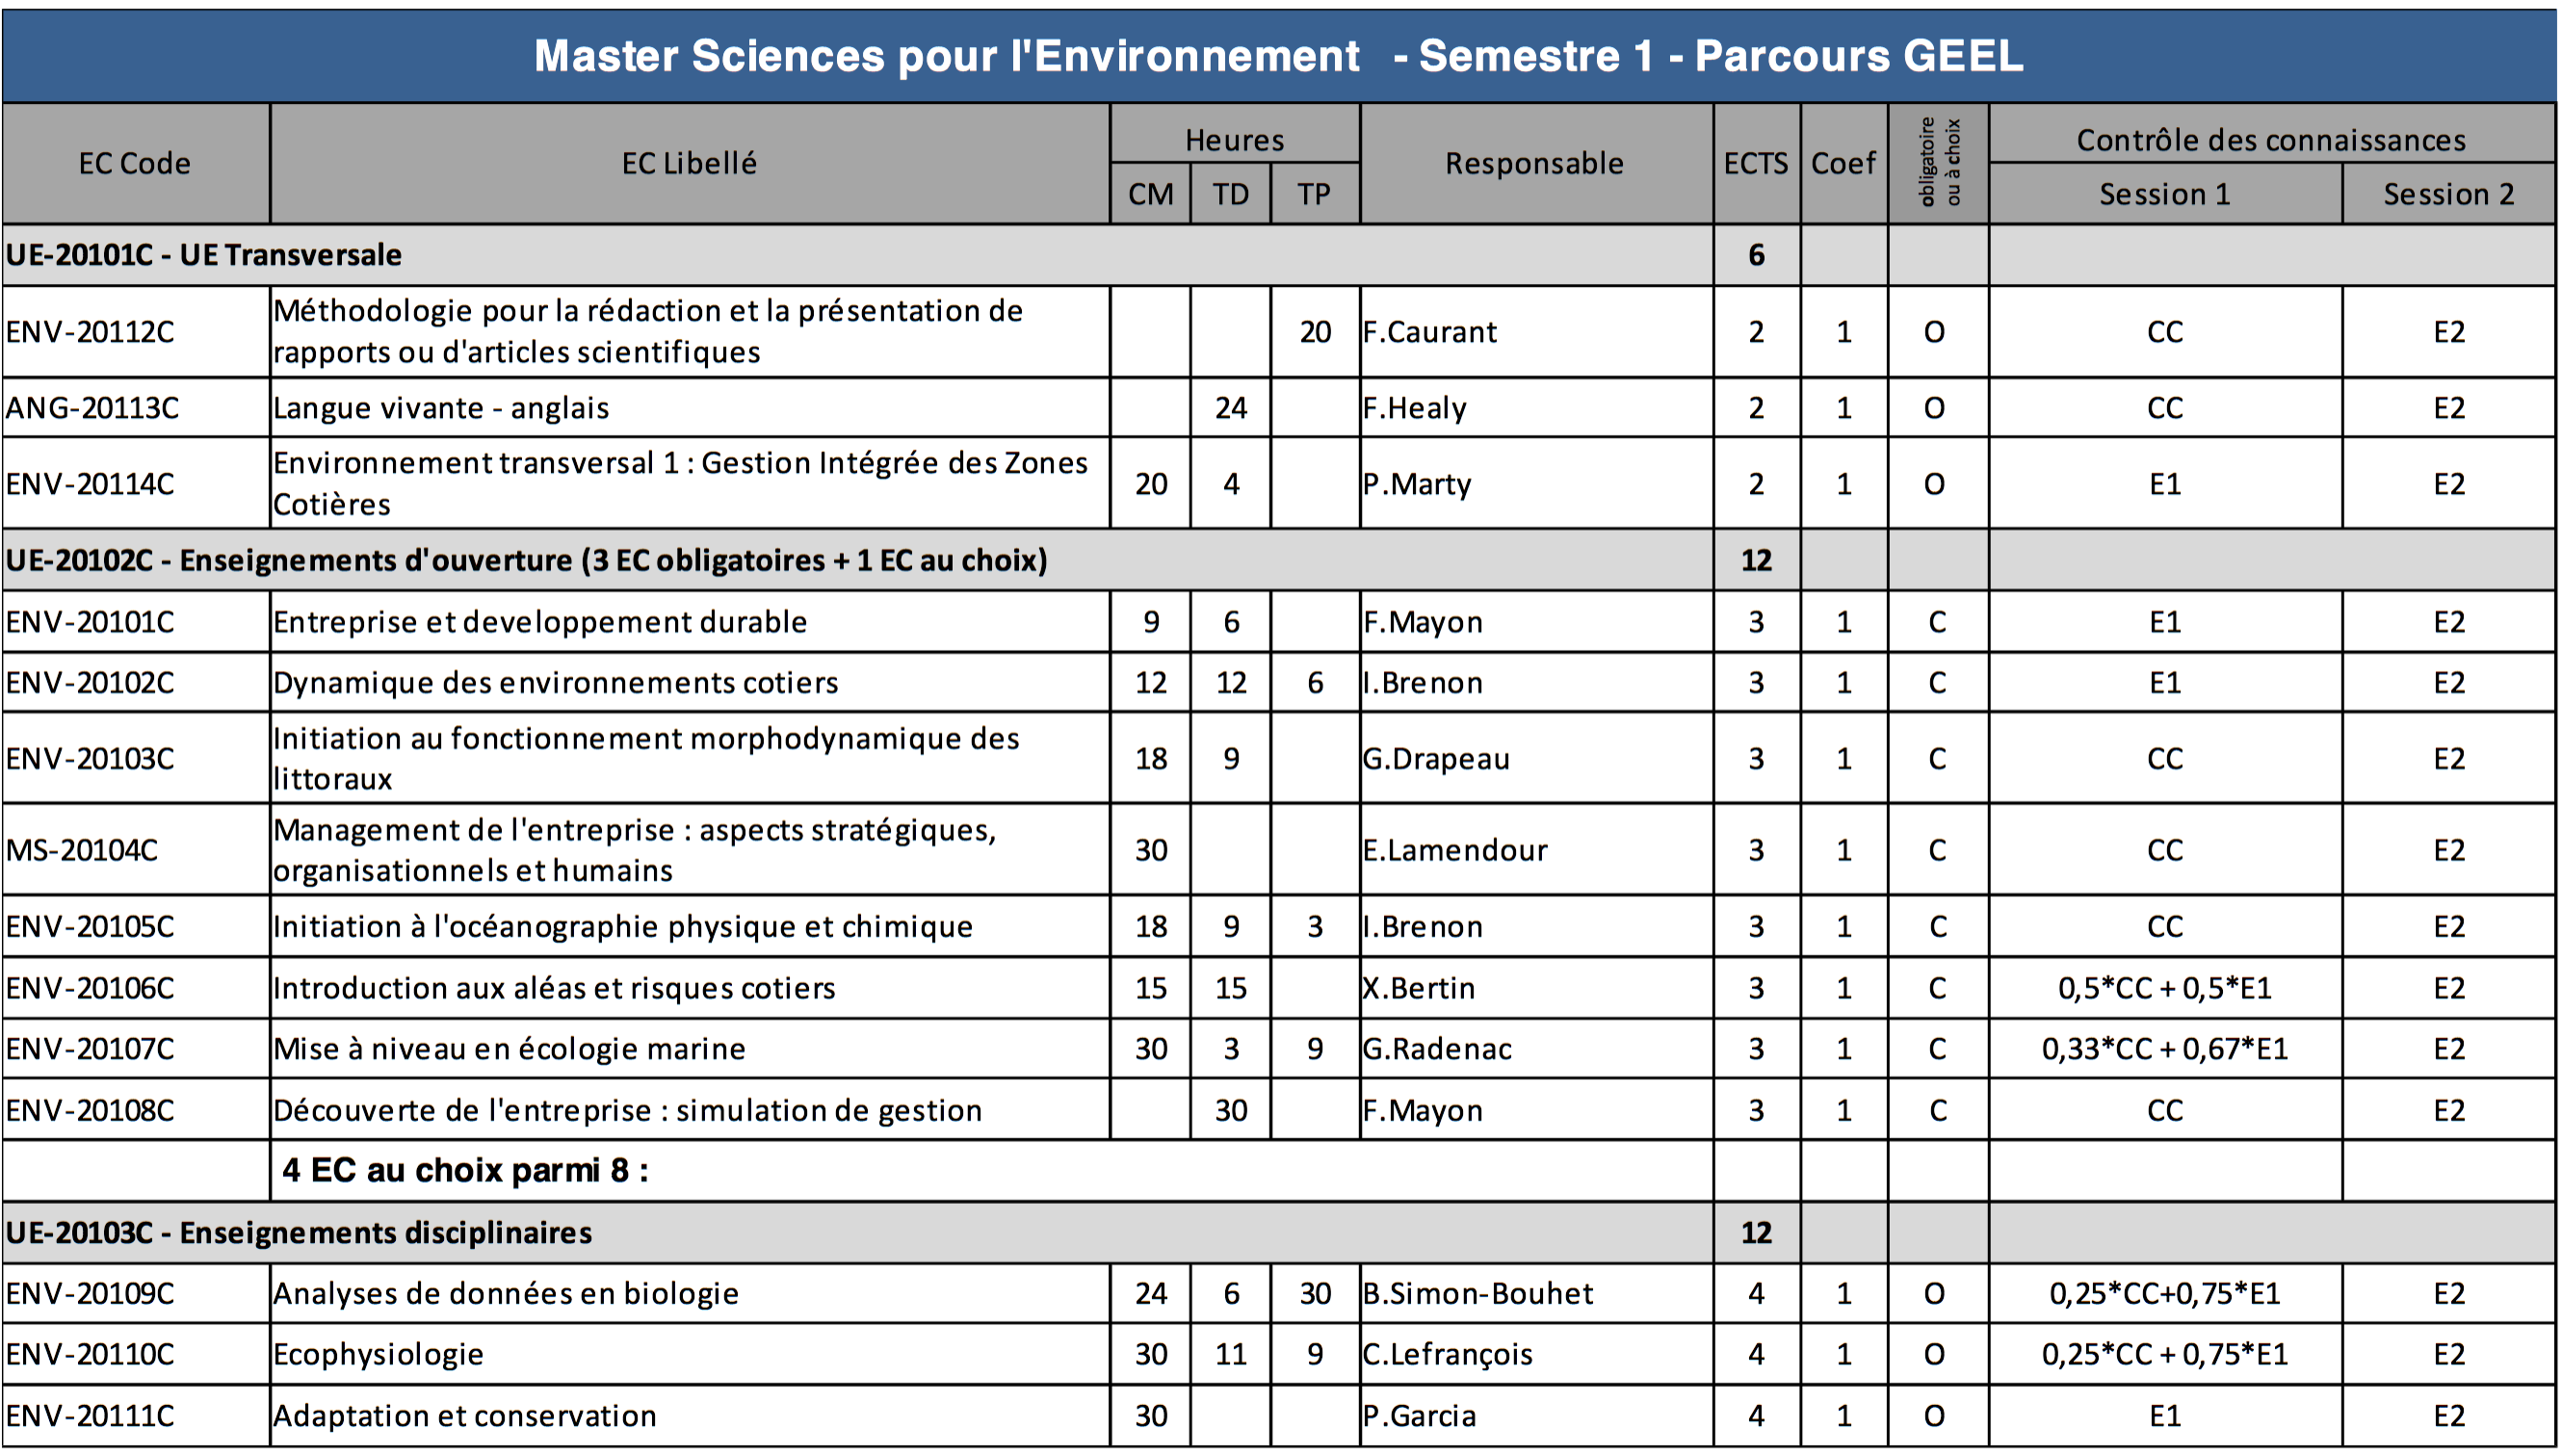
\includegraphics[width=\textwidth]{GEEL_S1.png}
\end{figure}

\FloatBarrier

\begin{figure}[htbp]
		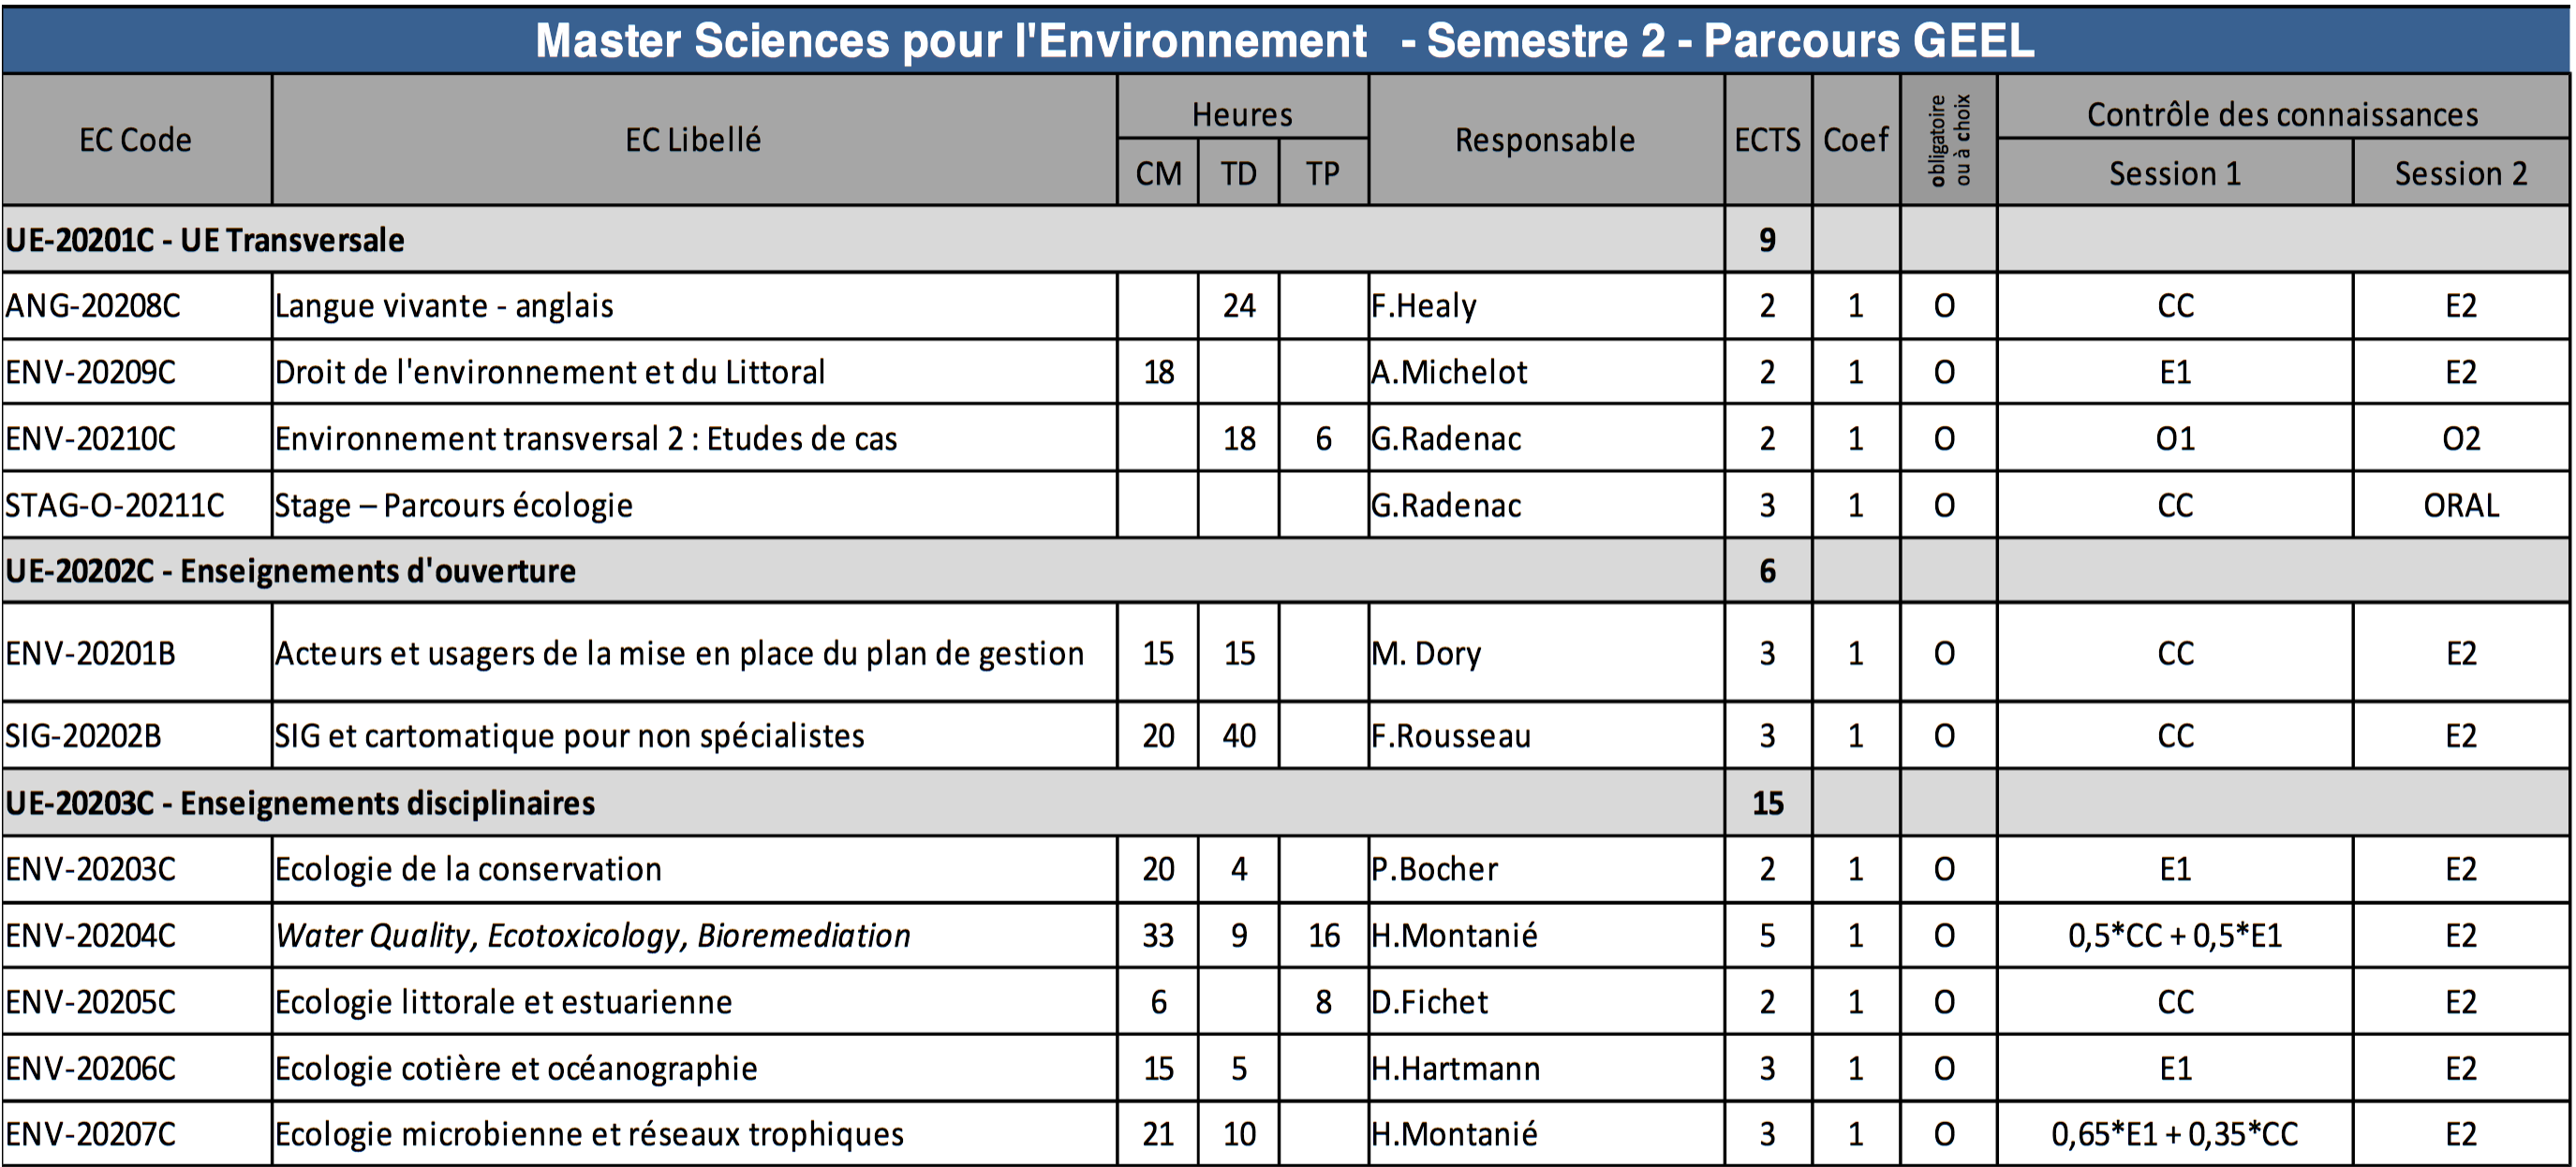
\includegraphics[width=\textwidth]{GEEL_S2.png}
\end{figure}

\FloatBarrier


\begin{sidewaystable}[]
\centering
\caption{My caption}
\label{my-label}
\resizebox{\linewidth}{!}{%
\begin{tabular}{lllllllllll}
\rowcolor[HTML]{9B9B9B} 
Semestre 1    &                                                                                           &    &    &    &                 &      &      &             &                   &           \\
\rowcolor[HTML]{C0C0C0} 
Code EC       & Libellé                                                                                   & CM & TD & TP & Responsable     & ECTS & Coef & Obligatoire & Session 1         & Session 2 \\
\rowcolor[HTML]{EFEFEF} 
UE-20101C     & UE transversale                                                                           &    &    &    &                 & 6    &      &             &                   &           \\
ENV-20112C    & Méthodologie pour la rédaction et la présentation de rapports ou d'articles scientifiques &    &    & 20 & F. Caurant      & 2    & 1    & O           & CC                & E2        \\
ANG-20113C    & Langue vivante - anglais                                                                  &    & 24 &    & F. Healy        & 2    & 1    & O           & CC                & E2        \\
ENV-20114C    & Environnement transversal 1 : Gestion Intégrée des Zones Côtières                         & 20 & 4  &    & C. Parain       & 2    & 1    & O           & E1                & E2        \\
\rowcolor[HTML]{EFEFEF} 
UE-20102C     & UE d'ouverture (3 EC obligatoires + 1 EC au choix)                                        &    &    &    &                 & 12   &      &             &                   &           \\
ENV-20101C    & Entreprise et développement durable                                                       & 9  & 6  &    & F. Mayon        & 3    & 1    & O           & E1                & E2        \\
ENV-20102C    & Dynamique des environnements côtiers                                                      & 12 & 12 & 6  & I. Brenon       & 3    & 1    & O           & E1                & E2        \\
ENV-20103C    & Initiation au fonctionnemet morphodynamique des littoraux                                 & 18 & 9  &    & V. Duvat-Magnan & 3    & 1    & O           & CC                & E2        \\
MS-20104C     & Management de l'entreprise : aspects stratégiques, organisationnels et humains            & 30 &    &    & E. Lamendour    & 3    & 1    & C           & CC                & E2        \\
ENV-20105C    & Initiation à l'océanographie physique et chimique                                         & 18 & 9  & 3  & I. Brenon       & 3    & 1    & C           & CC                & E2        \\
ENV-20106C    & Introduction aux aléas et risques côtiers                                                 & 15 & 15 &    & X. Bertin       & 3    & 1    & C           & 0,5*CC + 0,5*E1   & E2        \\
ENV-20107C    & Mise à niveau en écologie marine                                                          & 30 & 3  & 9  & G. Radenac      & 3    & 1    & C           & 0,33*CC + 0,67*E1 & E2        \\
ENV-20108C    & Découverte de l'entreprise : simulation de gestion                                        &    & 30 &    & F. Mayon        & 3    & 1    & C           & CC                & E2        \\
\rowcolor[HTML]{EFEFEF} 
UE-20103C     & UE disciplinaire                                                                          &    &    &    &                 & 12   &      &             &                   &           \\
ENV-20109C    & Analyse de données en biologie                                                            & 24 & 6  & 30 & B. Simon-Bouhet & 4    & 1    & O           & 0,25*CC + 0,75*E1 & E2        \\
ENV-20110C    & Écophysiologie                                                                            & 30 & 11 & 9  & C. Lefrançois   & 4    & 1    & O           & 0,25*CC + 0,75*E1 & E2        \\
ENV-20111C    & Adaptation et conservation                                                                & 30 &    &    & P. Garcia       & 4    & 1    & O           & E1                & E2        \\
\rowcolor[HTML]{9B9B9B} 
Semestre 2    &                                                                                           &    &    &    &                 &      &      &             &                   &           \\
\rowcolor[HTML]{C0C0C0} 
Code EC       & Libellé                                                                                   & CM & TD & TP & Responsable     & ECTS & Coef & Obligatoire & Session 1         & Session 2 \\
\rowcolor[HTML]{EFEFEF} 
UE-20201C     & UE transversale                                                                           &    &    &    &                 & 6    &      &             &                   &           \\
ANG-20208C    & Langue vivante - anglais                                                                  &    & 24 &    & F.Healy         & 2    & 1    & O           & CC                & E2        \\
ENV-20209C    & Droit de l'environnement et du Littoral                                                   & 18 &    &    & A.Michelot      & 2    & 1    & O           & E1                & E2        \\
ENV-20210C    & Environnement transversal 2 : Etudes de cas                                               &    & 18 & 6  & G.Radenac       & 2    & 1    & O           & O1                & O2        \\
\rowcolor[HTML]{EFEFEF} 
UE-20202C     & UE d'ouverture                                                                            &    &    &    &                 & 6    &      &             &                   &           \\
ENV-20201B    & Acteurs et usagers de la mise en place du plan de gestion                                 & 15 & 15 &    & M. Dory         & 3    & 1    & O           & CC                & E2        \\
SIG-20202B    & SIG et cartomatique pour non spécialistes                                                 & 20 & 40 &    & F.Rousseau      & 3    & 1    & O           & CC                & E2        \\
\rowcolor[HTML]{EFEFEF} 
UE-20203C     & UE disciplinaire                                                                          &    &    &    &                 & 18   &      &             &                   &           \\
ENV-20203C    & Ecologie de la conservation                                                               & 20 & 4  &    & P.Bocher        & 2    & 1    & O           & E1                & E2        \\
ENV-20204C    & Water Quality, Ecotoxicology, Bioremediation                                              & 33 & 9  & 16 & H.Montanié      & 5    & 1    & O           & 0,5*CC + 0,5*E1   & E2        \\
ENV-20205C    & Ecologie littorale et estuarienne                                                         & 6  &    & 8  & D.Fichet        & 2    & 1    & O           & CC                & E2        \\
ENV-20206C    & Ecologie cotière et océanographie                                                         & 15 & 5  &    & H.Hartmann      & 3    & 1    & O           & E1                & E2        \\
ENV-20207C    & Ecologie microbienne et réseaux trophiques                                                & 21 & 10 &    & H.Montanié      & 3    & 1    & O           & 0,65*E1 + 0,35*CC & E2        \\
STAG-O-20211C & Stage – Parcours écologie                                                                 &    &    &    & G.Radenac       & 3    & 1    & O           & CC                & ORAL      \\
\rowcolor[HTML]{9B9B9B} 
Semestre 3    &                                                                                           &    &    &    &                 &      &      &             &                   &           \\
\rowcolor[HTML]{C0C0C0} 
Code EC       & Libellé                                                                                   & CM & TD & TP & Responsable     & ECTS & Coef & Obligatoire & Session 1         & Session 2 \\
              & UE transversale                                                                           &    &    &    &                 &      &      &             &                   &           \\
              & Politiques publiques du développement durable                                             &    &    &    &                 &      &      &             &                   &           \\
              & Enjeux environnementaux et sociétaux                                                      &    &    &    &                 &      &      &             &                   &           \\
              & Analyse numérique                                                                         &    &    &    &                 &      &      &             &                   &           \\
              & SIG appliquée à l'environnement                                                           &    &    &    &                 &      &      &             &                   &           \\
              & Langue vivante - anglais                                                                  &    &    &    &                 &      &      &             &                   &           \\
              & UE disciplinaire                                                                          &    &    &    &                 &      &      &             &                   &          
\end{tabular}}
\end{sidewaystable}


=======
>>>>>>> master

\subsubsection{Semestres 3 et 4}


\subsection{GGL}

\subsubsection{Semestres 1 et 2}
<<<<<<< HEAD


=======


>>>>>>> master
\subsubsection{Semestres 3 et 4}


\subsection{GAGL}

\subsubsection{Semestres 1 et 2}
<<<<<<< HEAD


=======


>>>>>>> master
\subsubsection{Semestres 3 et 4}


\subsection{ME}

\subsubsection{Semestres 1 et 2}


\subsubsection{Semestres 3 et 4}


\section{Calendriers}\label{Calendrier}

\subsection{GEEL}

\subsubsection{M1}

\subsubsection{M2}


\subsection{GGL}

\subsubsection{M1}

\subsubsection{M2}


\subsection{GAGL}

\subsubsection{M1}

\subsubsection{M2}


\subsection{ME}

\subsubsection{M1}

\subsubsection{M2}

\end{document}
